\documentclass[10pt,a4paper]{article}
\usepackage[utf8]{inputenc}
\usepackage{amsmath}
\usepackage{amsfonts}
\usepackage{amssymb}
\usepackage{graphicx}
\usepackage{natbib}
%\usepackage{biblatex}
%\addbibresource{rf.bib}

%opening
\title{Random forests for facial recognition}
\author{Carl Ehrett}

\begin{document}

\maketitle

\section{What random forests are}\label{intro}

Random forests are an ensemble learning method that uses bagging in conjunction with random feature selection to reduce the variance of a decision tree estimator. Random forests are popular for their supposed resistance to overfitting and related low level of tuning required. Random forests often work well with ``out-of-the-box'' default settings, so that tuning is often a matter of coaxing fairly small improvements out of the model.

In this paper, I describe the nature and history of random forests in the remainder of Section \ref{intro}. I explore some of the benefits of random forests in Section \ref{benefits}. I also describe some of the grand claims that are often made about random forests, and explore the truth of those claims, in Section \ref{claims}. I demonstrate the use of random forests as a facial recognition classifier in Section \ref{application}. Throughout this paper, I will focus on the use of random forests as a classifier (which is the use for which random forests are more popular).

\subsection{Decision trees}
A decision tree is a partitioning of the feature space into hyperrectangles the edges of which are aligned with the axes of the feature space. The decision tree assigns to each subset of the partition a prediction value. If a tree is used for classification, then a point $x$ is classified as being in the category to which a plurality training samples belong in the subset to which $x$ belongs; for regression, $x$ is associated with the mean value of the samples in the subset. An example from \citet{Hastie2009} is shown in Figure \ref{fig:tree}, where a single tree is visualized in two different ways.
%
\begin{figure}
	\centering
	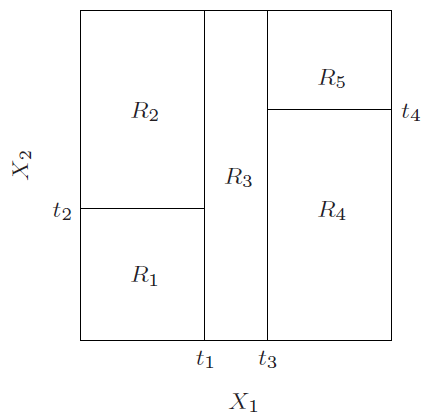
\includegraphics[width=0.45\linewidth]{CART1}\hspace{1cm} 
	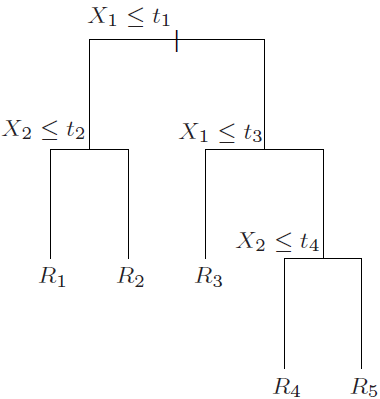
\includegraphics[width=0.45\linewidth]{CART2}
	\caption{Two representations of the same decision tree on a two-dimensional feature space, such as would be grown using the CART algorithm.}
	\label{fig:tree}
\end{figure}
%

The decision trees used in random forests are not required to be grown following any particular algorithm. The most common algorithm to use for this purpose is the CART algorithm \cite{Breiman1984}. All tuning parameters that apply to the decision trees used in random forests are, by extension, tuning parameters for random forests itself. For example, the maximum depth of trees can be tuned, or the minimum number of samples to include in each terminal node, or the minimum improvement (measured e.g. by Gini impurity) required to split a node.

\subsection{Bagging}
Bagging, or bootstrap aggregation, is a means for reducing the variance of an estimator by combining many versions of that estimator \citep{Breiman1996}. Suppose one has a method for producing an estimator $\hat f(x)$ at a point $x$ using some training data. To produce a bagged version of this estimator, one would do the following.
\begin{enumerate}
	\item Produce $B$ bootstrap samples of the training data.
	\item Fit the model on each bootstrap sample.
	\item Get a prediction $\hat f^{*b}(x)$  using each bootstrap sample fit $b=1,\ldots,B$.
	\item Combine all of these predictions. For regression, $\hat f_{\mathrm{bag}}(x)=\frac 1B \sum_{b=1}^B \hat f^{*b}(x)$, and for classification $\hat f_{\mathrm{bag}}(x) = \mathrm{argmax}_{k} \sum_{b=1}^B \mathbf1_{\hat f^{*b}(x)}$
\end{enumerate}

Bagging helps to address one of the primary drawbacks of decision trees: their high variance. The variance of an average of $B$ identically distributed variables with variance $\sigma^2$ and pairwise correlation $\rho$ is given by:
\begin{equation}\label{eqn:corr}
\rho \sigma^2 + \frac{1-\rho}B \sigma^2.
\end{equation}
The second term above is driven to 0 as $B\to\infty$.

\subsection{Random feature selection}
Notice that \eqref{eqn:corr} above shows that bagging can reduce only the second term in that expression. If $\sigma^2$ and $\rho$ are both high, then the resulting variance of the bagged estimator will itself remain high. Therefore, since decision trees do indeed suffer high variance, random forests include random feature selection to reduce the correlation amongst the trees in the forest.

The use of random feature selection in ensembles of decision trees was suggested by \citet{TinKamHo1995}. \citet{Breiman2001} combined this idea with bagging to produce the method that is now known (and indeed trademarked by Breiman and his colleague Adele Cutler) as random forests.

To employ random feature selection in growing a decision tree one does as follows. Each time a node is split when growing a decision tree, the splitting variable for that node is chosen from amongst a random subset of $m<p$ of the $p$ predictors. Breiman suggests a default of $m=\sqrt{p}$ for classification and $m=p/3$ for regression, but it is often profitable to tune $m$ rather than relying on these defaults. 

\section{OOB error and feature importances}\label{benefits}

By virtue of using bagging and decision trees, random forests boasts some features that improve the utility and interpretability of the technique, including out-of-bag error and methods for estimating feature importances.

\subsection{OOB error}

Out-of-bag (OOB) error is a means for estimating the generalization error of a random forest without needing either a test set or cross-validation. OOB error is available whenever one uses bagging, as in random forests. To find the OOB error after training a model, one tests each of the training samples $x_i$ using only the bagged models that do not include $x_i$ in the bootstrap sample set upon which that model was trained. For example, in the case of random forest classification, we would test $x_i$ by classifying it using all and only the trees that were grown from a bootstrap sample set which does not include $x_i$. These are the trees for which $x_i$ was ``out of the bag'' upon which the trees were trained.

The result is similar to cross-validation, which also involves testing each training sample $x_i$ on versions of the model that were trained on subsets of the training set that exclude $x_i$. Thus random forests provides an analogue to cross-validation that does not requires neither training the model multiple times, nor setting aside a portion of the data to serve as a test set.

\subsection{Feature importances}\label{feature_importances}

Decision trees are valued for their high interpretability. In contrast with ``black box'' methods such as neural nets, decision trees explicitly show how the covariates relate to the estimate. For example, in Figure \ref{fig:tree}, we can see that a point in the region $R_1$ gets the estimate that it does because $X_1 < t_1$ and because, as a point with $X_1 < t_1$, that point also has $X_2<t_2$. All such points, with $X_1<t_1$ and $X_2<t_2$, belong in region $R_1$ and receive a common estimate.

Though random forests are built from decision trees, this form of interpretability is lost through the bagging procedure. Though each tree in the forest remains interpretable in this way, the forest itself, as an average of trees, does not offer the same explicit guide to how a prediction point is assigned its estimate. This is a downside of using random forests instead of a single decision tree.

However, random forests can nonetheless regain some of this interpretability through other means. Specifically, various methods are available for estimating the relative importances of the predictor variables used in random forests. Three such methods are as follows:
\begin{enumerate}
	\item For each node split while growing a tree, record the improvement (e.g. measured via Gini impurity) generated by the split. For each covariate, average the improvements it produces each time it is used for a split \citep{Hastie2009}.
	\item For each tree, find the OOB error, then for each covariate measure the increase in OOB error when you randomly permute that covariate's values. Average these values across all trees \citep{Breiman2001}.
	\item For each node split, record the proportion of training samples that are “downstream” of that split. For each variable, find the average proportion of samples that are ``downstream" of its splits \citep{scikit-learn}.
\end{enumerate}
These methods can be combined. For example, \citet{scikit-learn} combine scores from the first and third methods above to estimate the relative importances of the covariates.

\section{Claims about random forests}\label{claims}

Thanks to neural nets, no other machine learning method needs to worry about being the most overhyped technique. However, it remains true that random forests are the subject of some fairly grand claims.

For example, \citeauthor{breiman_cutler} claim on their random forests website that ``[r]andom forests does not overfit.'' This claim is false; any learning method can overfit. See the example included in the RMarkdown document accompanying this paper for a simple case of overfitting by random forests. However, even in this pathological case which is designed specifically to cause overfitting, it remains true that the OOB error is a roughly unbiased estimate of the generalization error. Thus, even in a case in which random forests overfits, that overfitting may be easy to detect by comparing the OOB error to the training set prediction error.

The claim that random forests do not overfit has a grain of truth behind it. Namely, random forests do not overfit \emph{by virtue of growing too many trees}. Figure \ref{fig:error}, from \citet{Hastie2009}, shows a typical example of how test set error changes as a result of increasing $B$, the number of trees used in the forest. This simplifies the process of tuning random forests, since one need worry only about having ``enough'' trees, and not about having ``too many.''

\begin{figure}
	\centering
	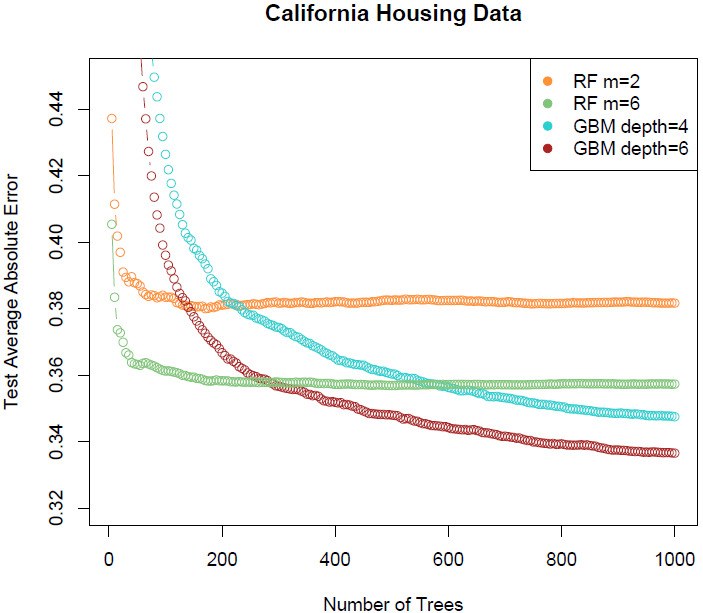
\includegraphics[width=0.8\linewidth]{comp3}
	\caption{Test error of two different random forest models (and two different gradient boosting models). Notice that the random forest test error appears to converge to its minimum.}
	\label{fig:error}
\end{figure}

Another claim made by Breiman and Cutler on their website is that, as a classifier, random forests are ``unexcelled in accuracy among current algorithms''. This is a difficult claim to assess (what exactly would constitute a demonstration of such a claim?), though Figure \ref{fig:error} is one of several examples that \citet{Hastie2009} describe in which random forests are outperformed by gradient boosting.

However, a reasonable stab at a comprehensive examination of the question of which classification algorithm is most accurate is undertaken by \citet{Fernandez-Delgado2014}. The authors evaluate 179 classifiers using 121 data sets. The authors find that the best performers on these 121 data sets are random forests, though their performance is not statistically significantly superior to that of support vector machines. Still, this study provides at least a substantive piece of support for the rather grand claim on Breiman and Cutler's website.

\section{Application}\label{application}

In this section I describe my application of random forests as a binary facial recognition model, which distinguishes whether a face belongs to myself or to my wife. The resulting model uses a very low number of covariates -- only thirty. The model is lightweight enough to operate in real time on webcam input, displaying the classification in real time as an overlay over the webcam image. It can furthermore classify multiple faces in the same image simultaneously.

To interact with my laptop's webcam, I employ the OpenCV Python library \citep{opencv_library}. To detect faces within the images gathered from the webcam, I employ the Dlib Python library \citep{King2009} in conjunction with the facial landmark database provided by \citet{Sagonas2016}. The Dlib-based Python approach I use is inspired by the drowsiness detection application described by \cite{Rosebrock2017}. The result of training Dlib's facial landmark detector on that data set is to produce a facial detector which returns the 2-D locations, within an image, of the 68 landmarks shown in Figure \ref{fig:landmarks}.
\begin{figure}
	\centering
	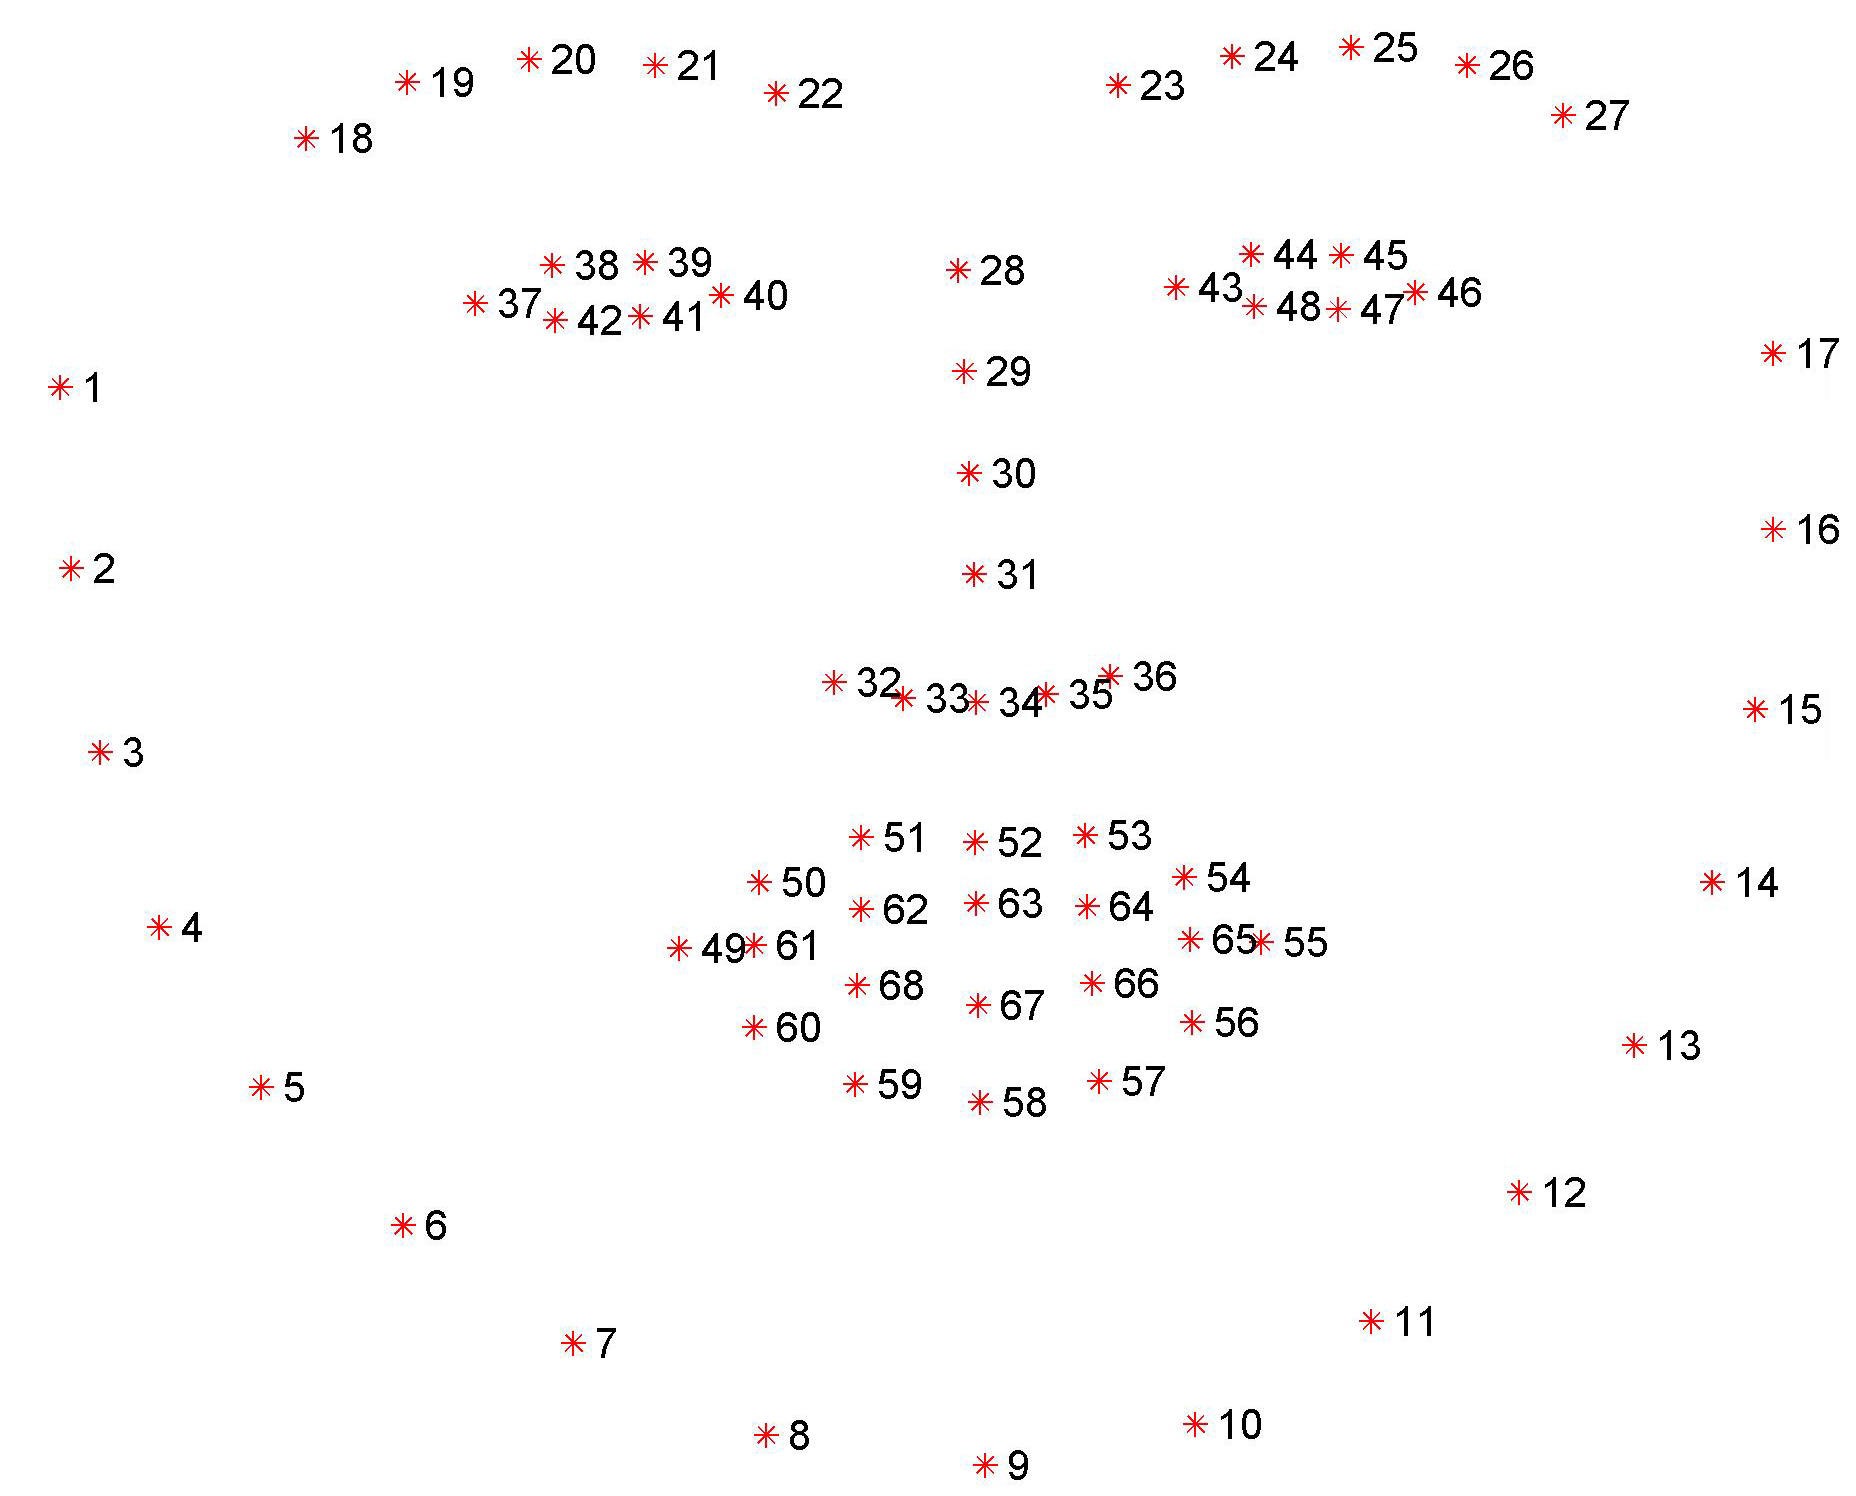
\includegraphics[width=0.8\linewidth]{figure_68_markup}
	\caption{68 facial landmarks. Image credit: \citet{Sagonas}.}
	\label{fig:landmarks}
\end{figure}

Using these 68 landmarks, I define 30 covariates. Each covariate is either a length (e.g. width of the lower jaw), an area of a triangle defined by three landmarks (e.g. each of the two sides of the nose), or an angle formed by three landmarks (e.g. temple to mouth to lower jaw). All covariates are measured after scaling the face to have length and width 1. For the precise definitions of the 30 covariates, see the Python code included as a supplement to this paper. Figure \ref{fig:covariates} shows an overlay which gives a sense of the covariates collected from each facial image.
\begin{figure}
	\centering
	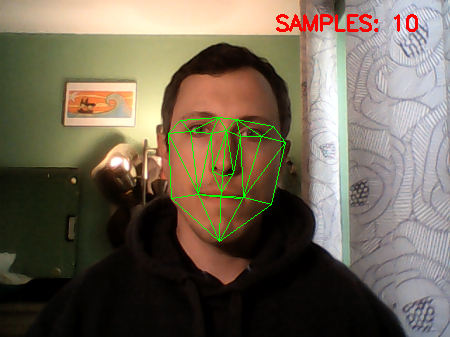
\includegraphics[width=0.8\linewidth]{00216}
	\caption{An image taken from the training samples of my face.}
	\label{fig:covariates}
\end{figure}
I collected 500 training samples each from myself and from my wife.

To fit the model, I used the implementation of random forests in the Scikit-learn Python library \citep{scikit-learn}. Default settings worked well, generating 6\% OOB error. After tuning, the model reached 3\% OOB error. The tuned model deviates from Scikit-learn's defaults only by increasing the number of trees from 10 to 100. Setting maximum tree depths and changing the number of predictors used in random feature selection (from the default of $\lfloor \sqrt p\rfloor=\lfloor \sqrt {30}\rfloor=5$) appeared to have either no effect, or deleterious effects upon the model.

The resulting model performs well on new webcam input, with an error rate similar to that suggested by the OOB error. The classifier is fast enough to operate in real time on webcam input. An example of the classifier in action is shown in Figure \ref{fig:faces}.
\begin{figure}
	\centering
	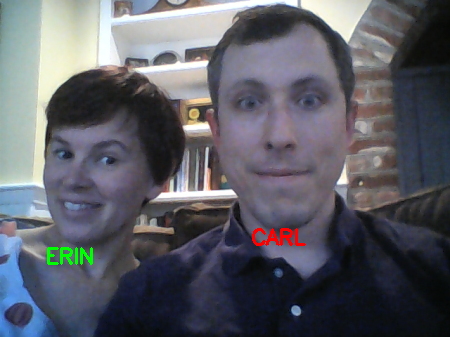
\includegraphics[width=0.8\linewidth]{00085}
	\caption{An example of the classifier in action, labelling multiple faces simultaneously on a real-time webcam feed.}
	\label{fig:faces}
\end{figure}

As described in Section \ref{feature_importances}, random forests can be used to estimate the relative importances of the predictors used in arriving at the classification predictions. The feature importances from the facial classifier are shown in Figure \ref{fig:feature_importances}.
\begin{figure}
	\centering
	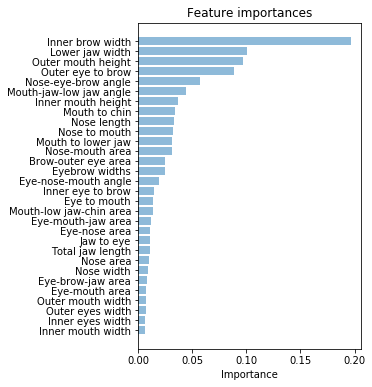
\includegraphics[width=0.8\linewidth]{feature_importances}
	\caption{Relative feature importances in the facial classifier.}
	\label{fig:feature_importances}
\end{figure}
An unexpected result is that inner brow width (the distance between the eyebrows) is by far the most important covariate distinguishing my face from my wife's. Lower jaw width is less surprising, but outer mouth height (the distance from the top of the upper lip to the bottom of the lower lip) is somewhat strange to find so high on this list. My suspicion is that this is an artifact of the data collection process. When I collected training samples from my own face, I was alone. When I collected samples from my wife's face, we were conversing. Therefore, the importance of outer mouth height is, I suspect, simply due to the fact that she was speaking in many of her training samples, whereas I was not.

\section{Conclusion}
Random forests are a robust method for regression and classification that work well with minimal tuning. They are resistant to (but not immune from) overfitting, and where they have overfit, this is generally detectable by relying on the OOB error. The OOB error provides an estimate of the generalization error without requiring a test set or cross-validation. Random forests sacrifice some of the interpretability of single trees, but they can still be used to explore the relative importances of the covariates used in the model. Random forests can be used to build a lightweight binary facial classifier that can operate in real time on webcam input with high accuracy.

It would be relatively easy to extend this application to more than two faces. It remains to be seen to what extent accuracy would suffer by doing so. It would also be interesting to explore different sets of covariates. Examination of Figure \ref{feature_importances} suggests that several covariates could be removed without undermining the model. It may also be profitable to add covariates not currently considered by the model. A useful approach would be to define a great many covariates, and then use random forests to estimate the feature importances of these covariates for variable selection.

\bibliographystyle{apalike}
\bibliography{rf}
\end{document}
